\documentclass[sigconf]{acmart}

\def\BibTeX{{\rm B\kern-.05em{\sc i\kern-.025em b}\kern-.08emT\kern-.1667em\lower.7ex\hbox{E}\kern-.125emX}}
\usepackage{subfigure}
\usepackage{algorithm}
%\usepackage{algorithmic}
\usepackage{algpseudocode}
\usepackage{amsmath}
\usepackage{graphics}
\usepackage{epsfig}
\usepackage{multirow}
\usepackage{graphicx}
\usepackage{subfigure}

\renewcommand{\algorithmicrequire}{\textbf{Input:}} % Use Input in the format of Algorithm
\renewcommand{\algorithmicensure}{\textbf{Output:}} % Use Output in the format of Algorithm

\begin{document}

\title{Approximate Code: A Cost-Effective Erasure Coding Framework for Video Applications in Cloud Storage Systems}

\author{Huayi Jin}


%-------------------------ATTANTION-------------------------%
%                                                           %
% orange words show the content that requires to be add     %
% blue words need to be perfected or changed                %
% gray words are the placeholder which is easy to fill      %
%                                                           %
%-----------------------------------------------------------%

\begin{abstract}
Nowadays massive video data are stored in cloud storage systems, which are generated by various applications such as autonomous driving, news media, security monitoring, etc. Meanwhile, erasure coding is a popular technique in cloud storage to provide both high reliability with low monetary cost, where triple disk failure tolerant arrays (3DFTs) is a typical choice. Therefore, how to minimize the storage cost of video data in 3DFTs is challenge for cloud storage systems. Although there are several solutions like approximate storage technique for storage devices, it cannot guarantee low storage cost and high data reliability in storage systems concurrently.

To address this problem, in this paper, we propose Approximate Code, which is an erasure coding framework for video applications in cloud storage systems. The key idea of Approximate Code is distinguishing the important data and unimportant data in videos with different capabilities of fault tolerance. On one hand, for important data, Approximate Code provides triple parities to provide high reliability. On the other hand, single/double parities are applied for unimportant data, which can save the storage cost and accelerate the recovery process. To demonstrate the effectiveness of Approximate Code, we conduct several experiments in Hadoop systems. The results show that, compared to traditional 3DFTs using various erasure codes such as RS, STAR and TIP-Code, Approximate Code reduces the number of parities by up to 60\%, saves the storage cost by up to 10\%, increase the recovery speed by up to 1.5X when single disk fails, and can reconstruct the whole video data via fuzzification when triple disks fail.

\end{abstract}

%
% The code below is generated by the tool at http://dl.acm.org/ccs.cfm.
% Please copy and paste the code instead of the example below.
%
\keywords{Erasure Codes, Approximate Storage, Multimedia, Cloud Storage}

\maketitle

\section{Introduction}
For typical cloud storage systems such as Windows Azure [CITE] and Amazon AWS [CITE], erasure coding is a popular technique to provide both high reliability and low monetary cost [CITE EC], where triple disk failure fault tolerant arrays (3DFTs) are widely used. Typical erasure codes can be divided into two categories, RS-based Codes [CITE] and XOR-based codes [CITE]. RS-based codes [CITE] are encoded according the Galois Field Computation in Reed Solomon Code [CITE], which allow flexible configuration and have a little higher computation cost. XOR-based codes [CITE] simplify the computation, but the scalability is a significant issue in previous literatures.

With the increasing demand on higher resolution and frame rate for video data, tremendous storage devices are highly desired in cloud storage systems, which makes data centers much bigger. On YouTube, nearly 140,000 hours of video are played every minute and 400 hours of video are uploaded [DESCRIBE AND CITE YOUTUBE]. Therefore, in this paper, we set out to answer the following question,
In a cloud storage system, how to efficiently store the tremendous video data in 3DFTs?

To reduce the storage cost in cloud storage systems, a feasible solution is approximate storage. [DESCRIBE AND CITE APPROXIMATE STORAGE] but the data reliability cannot be guaranteed. Another solution is using disk arrays like RAID-5 or RAID-6 [CITE RAID], but the capability of fault tolerance should be sacrificed. Therefore, existing solutions cannot provide low storage cost and high reliability simultaneously.

To address the above problem, in this paper, we propose Approximate Code, which is an erasure coding framework to provide comprehensive solution for video data storage in cloud systems. The key idea of Approximate Code is treating the important/unimportant data in different ways. For important data, we add additional parities to provide high capability of fault tolerance. On the other hand, the unimportant data are encoded with a minimum number of parities, which only supply the basic requirement of the recovery. When triple disks fail, the lost data can be reconstructed via a fuzzy manner.

We have the following contributions of this work,
\begin{enumerate}
\item We propose Approximate Code, which a cost-effective framework to store video data in cloud storage systems.
\item Approximate Code can be implemented by combining most erasure codes in 3DFTs, such as RS, STAR Code, TIP-Code, etc.
\item We conduct several quantitative analysis, simulations and experiments according to different layouts of various erasure codes, and the results show that Approximate Code achieves lower storage cost and faster data recovery when single disk fails.
\end{enumerate}

The rest of the paper is organized as follows. In Section \ref{RelatedWork}, we introduce related work and our motivation. 
In Section \ref{ApCode}, the design of Approximate Code and its encoding and decoding process will be illustrated in detail. 
Section \ref{Implementation} introduce the implementation of our design, and section \ref{ap-recovery} analysis the performance of approximate video storage.
The evaluation is presented in Section \ref{evaluation} and the conclusion of our work is in Section \ref{Conclusion}. 

\section{Related Work and Our Motivation}\label{RelatedWork}
This section presents background on erasure codes, related video storage methods, approximate storage, and our motivation.

\iffalse
\begin{table}[]
\begin{tabular}{|c|l|}
\hline
Symbols & Description                          \\ \hline\hline
$n$     & the number of chunks in a stripe     \\ \hline
$m$     & the number of parity chunks          \\ \hline
$r$     & the number of sectors in a chunk     \\ \hline
$s$     & the number of columns of $D_I$       \\ \hline
$t$     & the number of rows of $D_I$          \\ \hline
$D_I$   & the zone of important data sectors   \\ \hline
$D_M$   & the zone of unimportant data sectors       \\ \hline
$Q$     & the zone of important parity sectors \\ \hline
$P$     & the zone of unimportant parity sectors     \\ \hline
\end{tabular}
\end{table}
\fi

\subsection{Existing Erasure Codes}

Reed Solomon Code (RS code) is a kind of Maximum Distance Separable (MDS) Codes, which have the optimal storage efficiency. The encoding and decoding operations of RS code are based on Galois Field, which leads to a higher computational complexity comparing to XOR-based codes.

However, due to its high scalability, RS code has been widely applied in traditional cloud storage systems. In a RS code which is delegated by RS($k$, $r$), $n = k + r$ denotes the total number
of nodes participating in the erasure coding schema, $k$ stands for the number of data nodes, and $r$ is the number of parity nodes. Generally data is organized and encoded/decoded with the minimum coding unit block. RS($k$, $r$) can tolerate at most $r$ failures at the same time, and single node failure can be recovered from any $k$ survivors. The encoding case of RS code and the failure tolerance processus are shown in Figure 1.


\begin{figure}[ht]
\centering
\begin{minipage}[b]{0.3\textwidth}
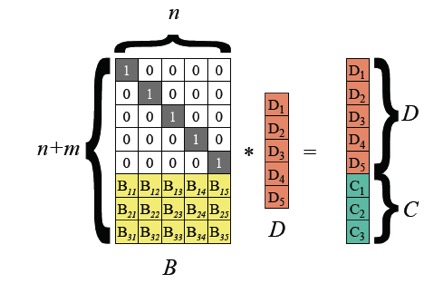
\includegraphics[width=0.52\textwidth]{photo/RS1.jpg}
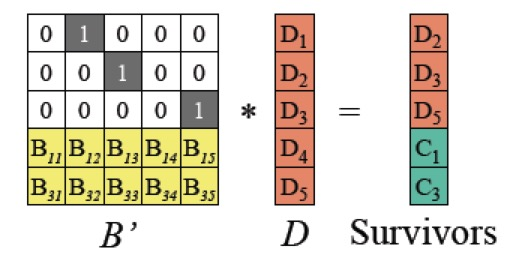
\includegraphics[width=0.4\textwidth]{photo/RS2.jpg}
\end{minipage}
\caption{Encoding process of RS($5$, $3$)}
\end{figure}

\begin{figure}[H]
\centering
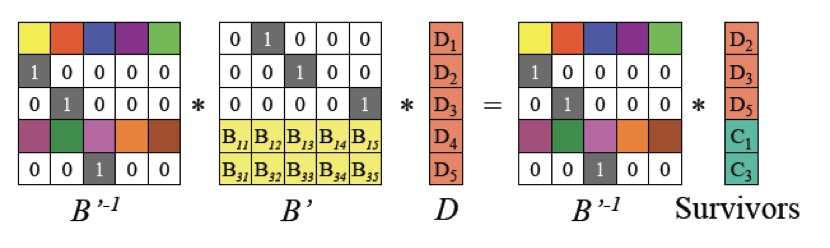
\includegraphics[width=0.3\textwidth]{photo/RS3.jpg}
\caption{Recovery processing of RS($5$, $3$) in the case of 3 random failure}
\end{figure}

\textcolor{red}{In our case, RS code could be applied. As the important data are uniformly-distributed in every node, the data in every node could be considered independent to each other. The principal of video storage divides the data into a small part of important frame and other subordinate frames. If a storage failure occurs in a node that stores largely the important frame, the data recovery may not be complete because the loss of the important frame could lead to a video quality degradation. In this way, this kind of uniformly-distribution would not allow the failure causing the data loss bigger than expected.}

\textcolor{red}{The data distribution assures the independency of nodes, the recovery of data could follow nearly the theoretical case. The recovery processus need the reversible matrix of original matrix. The calculation is shown in Figure 2.}

Another type of erasure code worth mentioning is XOR based codes, which uses purely XOR operations. There are two different approaches to implement XOR codes. One is to use generator matrix\cite{plank2004practical} for encoding/decoding operations, and the other is done by using specific algorithm for each code\cite{huang2008star}. In nowadays cloud storage systems, erasure codes for correcting two or three disk failures are widely used to ensure the reliability, and XOR-based codes show great advantages on encoding/decoding speed when the storage system is recovering from failures. XOR-based codes can be further categorized as XOR-based codes used in RAID-6 and ones to backup triple disk failure.

When it comes to RAID-6, Maximum Distance Separable (MDS) \cite{jin2009p} \cite{cassuto2009cyclic} \cite{blaum1999lowest} \cite{corbett2004row} \cite{blaum1995evenodd} \cite{bloemer1995xor} codes are frequently discussed. There are two types of MDS codes with different properties. One of them is called horizontal MDS codes, but it suffers from high write complexity and unbalanced I/O distribution. Accordingly, the other is called vertical MDS codes which has a common disadvantage of having resource-consuming partial strip write to continuous data.

A novel and efficient XOR-based RAID-6 code, named hybrid code(h-code) \cite{inproceedings}, is introduced a few years ago. This type of codes exploits the benefits of both horizontal and vertical MDS codes, therefore achieving optimization of partial stripe writes for RAID-6 in addition. H code can be applied to any array of (p+1) disks, where p is a prime number. The parities in H-Code are typical row parity and anti-diagonal parity. H-code does not have a specialized anti-diagonal parity strip, while it distributes the anti-diagonal parity elements among all the disks. Its horizontal parity ensures a partial stripe write to continuous data elements in a row share the same row parity chain, which achieves optimal partial stripe write performance. H code can be applied to any array of (p+1) disks, where p is a prime number. The analysis shows that H-Code achieves excellent performance in storage efficiency, encoding/decoding computational complexity and single write complexity. 


\subsection{Video Storage}\label{video storage}
For normal HD (resolution 1280$\times$720, 8-bit, 30 fps) video, the amount of raw video data in 1 minute is 4.63 GB, so video data is usually encoded and compressed before storage. Lossy compression is a common method that provides a much lower compression ratio than lossless compression while ensuring tolerable loss of video quality, and that is why we focus on such algorithms.


H.264 is one of the advanced algorithms for this type of work. This coding technique is widely used on platforms such as YouTube because it has higher compression ratio and lower complexity than its predecessor. For the HD video mentioned earlier, H.264 can reduce its size by about 10 times, only 443.27MB.

H.264 classifies all frames into three different categories:
\begin{enumerate}
    \item I frame: A frame that does not depend on other frame data, which means it can be decoded independently of other frames.
    \item P frame: A frame holds the changes compared to the previous frame, thus saving much space by leaving out redundant information.
    \item B frame: A frame saves more space by utilizing the data of both the preceding and following frame.
\end{enumerate}
In order to prevent the circumstance where a P or B frame references another distant frame, the concept of GOP is introduced. A GOP consists of multiple consecutive I,P and B frames which are independent of the frames in other GOPs. In other words, a P or B frame can only reference the ones inside the GOP which it belongs to, as shown in Figure \ref{H264-IPB}.
\begin{figure}[ht]
\centering
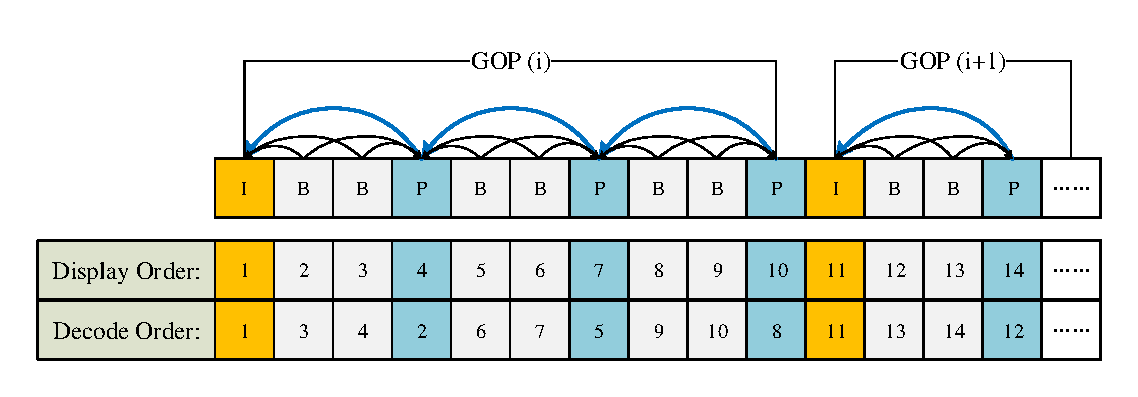
\includegraphics[width=0.45\textwidth]{photo/H264_IPB.pdf}
\caption{A sample of GOPs in H.264}
\label{H264-IPB}
\end{figure}


\subsubsection{Video Frame Recovery}

In the circumstance of video approximate storage, it's common to lose some frames and leave the video incomplete. However, the lost frames may still be recoverable with the benefit of nowadays powerful deep learning techniques. One of them is named video frame interpolation.

Video frame interpolation is one of the basic video processing techniques, an attempt to synthetically produce one or more intermediate video frames from existing ones, the simple case being the interpolation of one frame given two consecutive video frames. This is a technique that can model natural motion within a video, and generate frames according to this modelling. Artificially increasing the frame-rate of videos enables the possibility of frame recovery.


In deep learning methods, optical changes between the frames are trained in a supervised setup mapping two frames to their ground truth optical flow. Among all these, a multi-scale network\cite{van2017frame} based on recent advances in spatial transformers and composite perceptual losses as well as a context-aware Synthesis approach\cite{niklaus2018context} have so far produced the new state-of-the-art results in terms of PSNR and middlebury benchmark respectively.


The methods are relied on the completeness of some video frame, which enhances the importance of the only intact type of frame data in commonly used H.264 standard: the I frame.


\subsection{Approximate Storage}
Storage techniques nowadays generally regard all information of the same importance, which causes significant costs in energy, disk drives and computing resources. But not all data need high-reliability storage for its backup. That is when the concept of approximate storage is introduced. Approximate Storage is another way outside of traditional methods of trading off the limited resource budget with the costly reliability requirements, which recently receives more attentions since data centers are faced with storage pressure from the ever-increasing data.

Use cases for approximate storage range from transient memory to embedded settings and mass storage cloud servers. Mapping approximate data onto blocks that have exhausted their hardware error correction resources, for example, to extend memory endurance. On embedded settings, it enables the reduction of the cost of accesses and preserve battery life to loosen the capacity constraints. \cite{sampson2014approximate} Here, in data-center-scale video database, approximate storage can provide multiple levels of fault tolerance for data of different importance, avoiding redundant backup for the less-important data, thus saving a significant amount of space.


Approximate storage loosens the requirement of storage reliability by allowing quality loss of some specific data. Therefore, programmers can specify the importance of the data segments and assign them to different storage blocks. The critical data is still safe because they are stored and sufficiently backed up by expensive and highly reliable storage devices. Meanwhile, non-critical data is exposed to error, thus increasing storage density and saving cost.


However, it is too naive to store data in approximate storage units indiscriminately. Related research \cite{guo2016high} shows that this can lead to unacceptable data pollution. To ensure data quality in this case, higher error correction costs are required resulting in an increase in overall storage costs.


In the storage of video data, as described in \ref{video storage}, the I frame is the key to decoding the entire GOP. An error in the I frame will cause a decoding error in the P frames and the B frames, and the data loss of the I frame will cause the entire GOP to fail. In contrast, the error or loss of a P frame has less impact, while the B frame is most tolerant of errors because no other frames depend on it.

Considering the vital role the I frame plays in the video coding, we therefore define I frame data as the critical data of a video file. Although some part of P frames may play a relatively important role in the decoding process of a video, it’s importance can not exceed that of the I frames.

\begin{table}[ht]
\centering 
\caption{Comparison of fault tolerance and storage overhead between approximate storage, EC and Approximate Code}\label{tab-AS-EC-AP}
\begin{tabular}{|c|c|c|c|c|}
\hline
\multicolumn{2}{|c|}{Schemes}  & \begin{tabular}[c]{@{}c@{}}Storage\\ Overhead\end{tabular} & Realibilities & Performance \\ \hline\hline
\multirow{2}{*}{EC} & RS & high & high & medium \\ \cline{2-5} 
\multicolumn{1}{|c|}{} & RAID 6 & medium & medium & high \\ \hline
\multicolumn{2}{|c|}{Ap-Storage}& low & low & high \\ \hline
\multirow{2}{*}{Ap-Code}& Imp & \multirow{2}{*}{low} & high & high \\ \cline{2-2} \cline{4-5} 
 & unimportant &  & medium & high \\ \hline
\end{tabular}
\end{table}

\subsection{Our Motivation}
Based on Table \ref{tab-AS-EC-AP}, either the existing erasure codes or the approximate storage methods cannot meet the requirements of video applications in the cloud storage system due to the following reasons. 

First, existing erasure codes generally reach or exceed 3DFTs, and use more than 3 parity disks. However, the simultaneous damage of 3 disks is very rare, and the storage overhead paid for this is too large. Second, the existing erasure codes provide the same fault tolerance for all data without distinction, which results in the same reliability of important data that is sensitive to errors and data that is robust. Last but not least, the current approximate storage methods are unreliable since they are not designed to tolerate disk level failure.

To solve these problems, we propose a new erasure code called Approximation Code. It provides different fault tolerance for important and non-critical data to reduce storage overhead and protect critical data better.

\section{Approximate Code}\label{ApCode}
In this section, we introduce the design of Approximate Code and its properties through a few simple examples. 

The construction of the Approximate Code is determined by 3 parameters $k$, $r$ and $h$. 
First, we use Figure \ref{fig-chunk-block} to illustrate the term \emph{chunk}, \emph{block} and \emph{stripe} we use in this paper. In a $n$-node system, $k$ of them are data nodes and $r=n-k$ nodes are for parity. Each node can be divided into multiple blocks. We focus on the $s$ blocks of the same logical position of each node, and we treat these $s$ nodes as a \emph{chunk}. The $n$ chunks constitute a \emph{stripe}. 
Approximate Code are designed for $h$ stripes, where each stripe is in the same $n$-node system.
%Approximate Code are designed for $h$ stripes, where each stripe can be in the same $n$-node system, or on different $n$-node systems.
%We define the former situation as \emph{Situation I}, which we pay more attantion on, while the latter is defined as \emph{Situation II}.

\begin{figure}[ht]
\centering
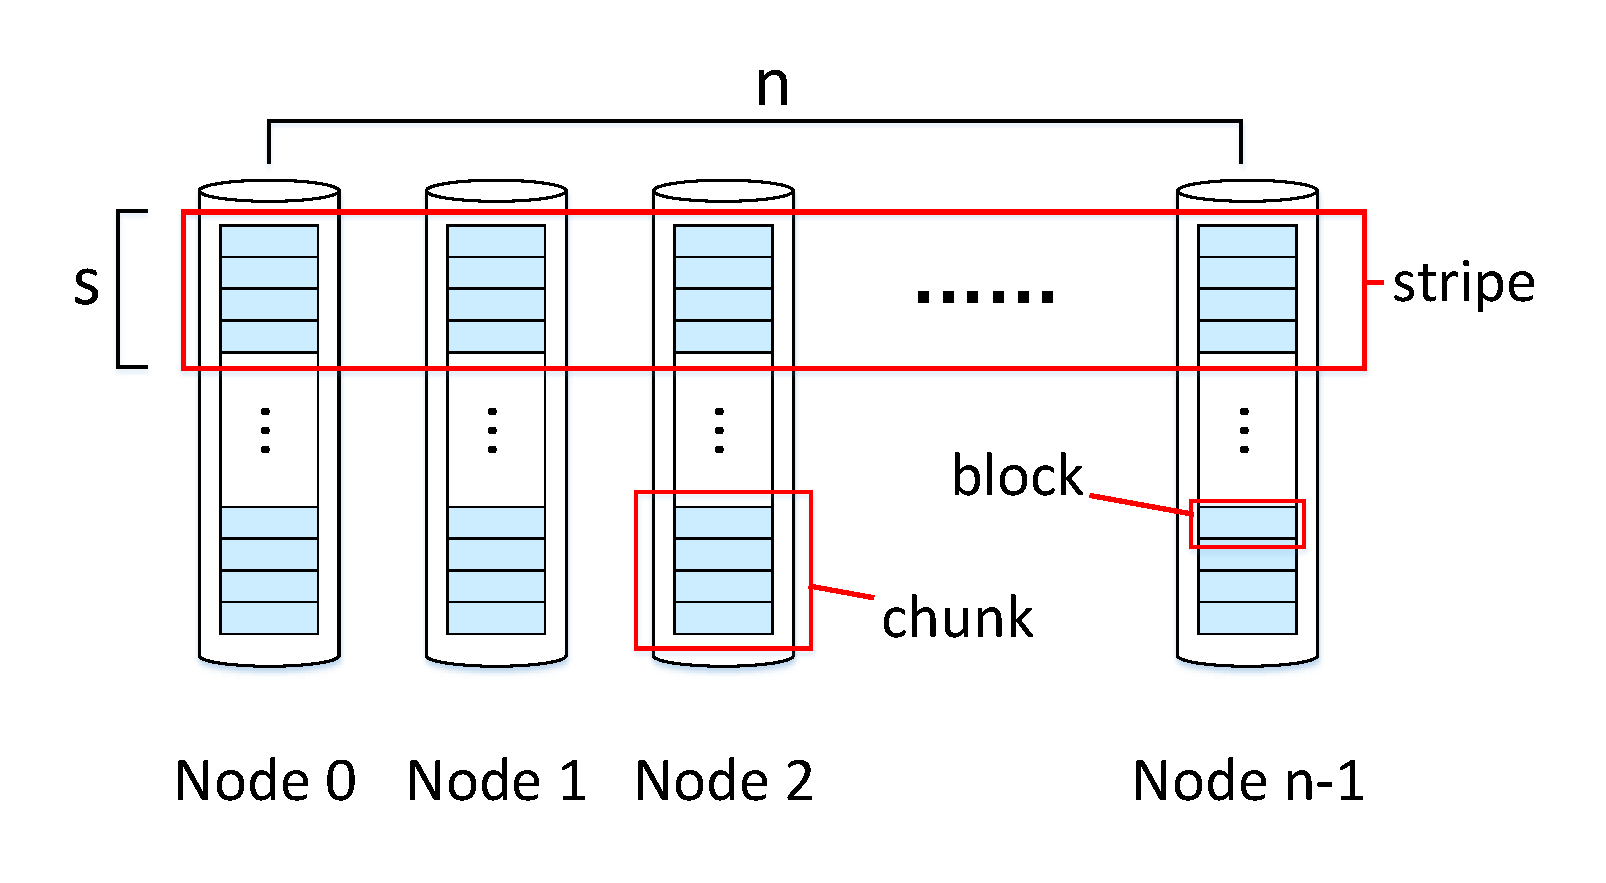
\includegraphics[width=0.35\textwidth]{photo/chunk-block.pdf}
\caption{A sample of chunks, stripes and blocks}
\label{fig-chunk-block}
\end{figure}

\subsection{Design of Approximate Code}
Approximate Code distribute important and unimportant data separately and mainly in two structure. As shown in Figure \ref{fig-ap-414}, in \emph{Structure 1}, important data occupies 1 of $s$ blocks in each chunk, and in \emph{Structure 2}, it occupies 1 of all $h$ data stripes.
We define that $h=s$, so in \emph{Structure 1} and \emph{Structure 2},important data accounts for $1/h$ of all data.

In each stripe, $r$ chunks are local parity chunks, which is encoded by the rest $k$ data chunks in the stripe.
In addition, there are another $3-r$ global chunks, which are calculated only by the important data blocks. It should be point out that the global parity chunks should be placed in different nodes and should be different from the data nodes. 

The number of important data blocks is $h \times k$, and they generate $h \times (3-r)$ global parity blocks.
To sum up, the number of blocks involved in the approximate code is 
$$(k+r)h^2 + (3-r) h$$


Approximate Code guarantees that for each stripe, the unimportant data can tolerate any $r$ node failures. Usually, $r$ is equal to 1 or 2, which covers most node failure scenarios, while important data are provided 3DFTs.

The construction of Approximate Code (4,1,4, \emph{Structure 1}) and Approximate (3,1,3, \emph{Structure 2}) can be illustrated by Figure \ref{fig-ap-414},

%As mentioned before, if it is considered that the chunks from the same column belong to the same node, this example includes 4 stripes with 7 nodes; otherwise, it includes 4 stripes with 22 nodes.

\begin{figure}[h]
\centering
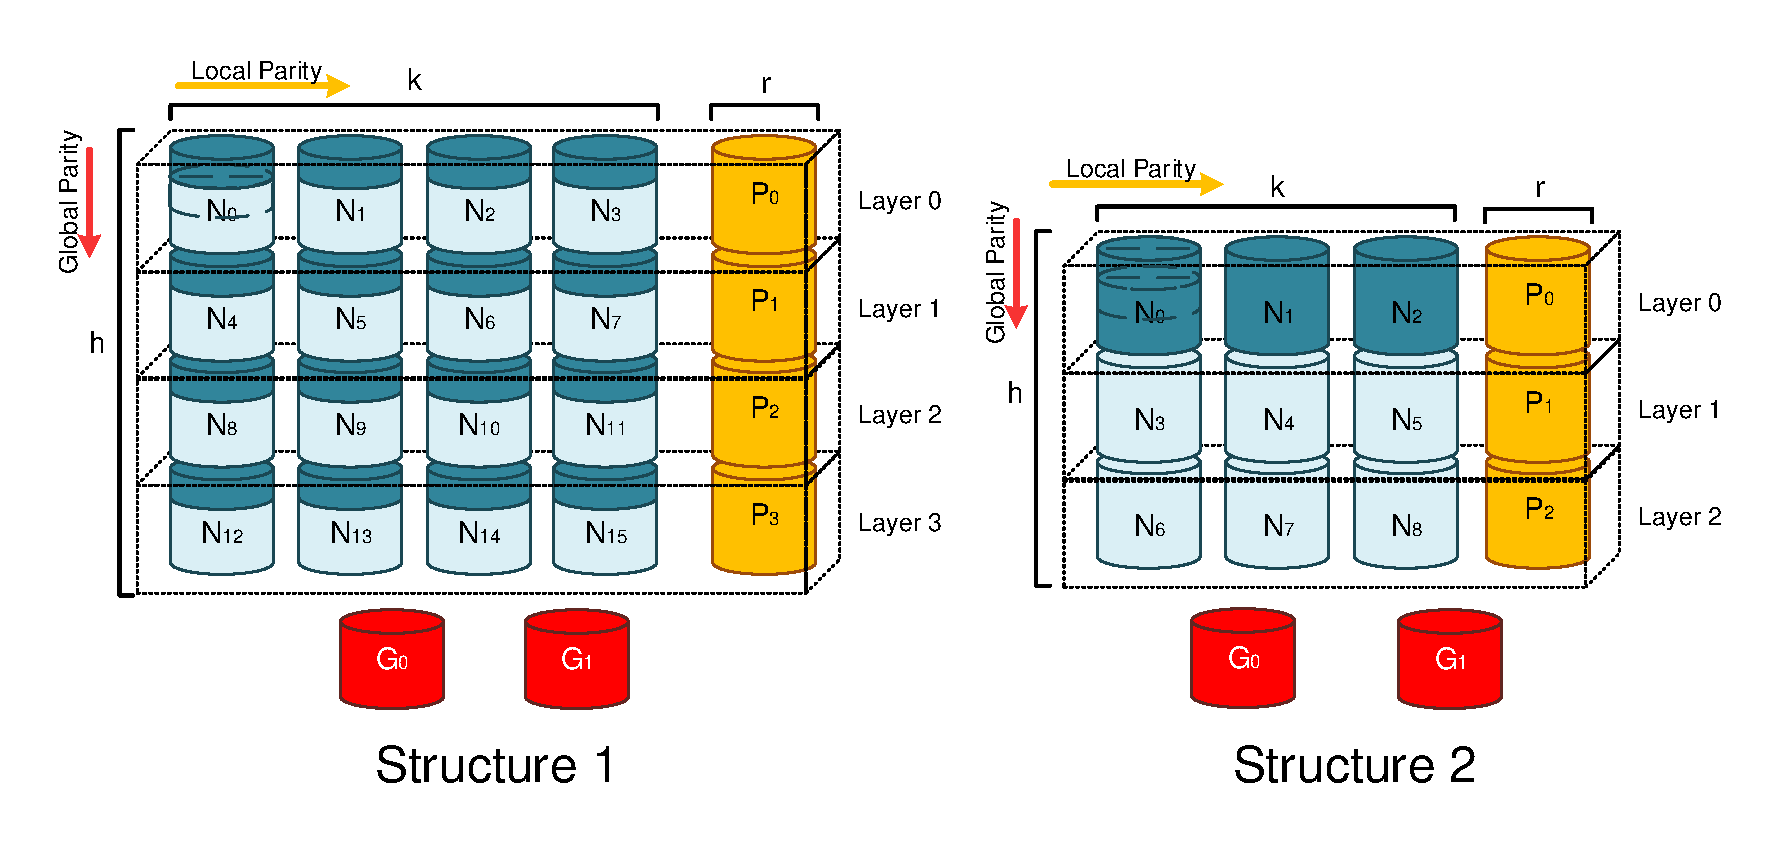
\includegraphics[width=\linewidth]{photo/AP-kmha-v7.pdf}
\caption{A sample of Approximate Codes $(4,1,4)$ in \emph{Structure 1}, and Approximate Code $(3,1,3)$ in \emph{Structure 2}.
Data chunks are marked as $N_i$, important data are marked as water green, local parity chunks are marked as orange and global parity chunks are marked as red.
}
\label{fig-ap-414}
\end{figure}

\begin{figure}[htb]
\centering
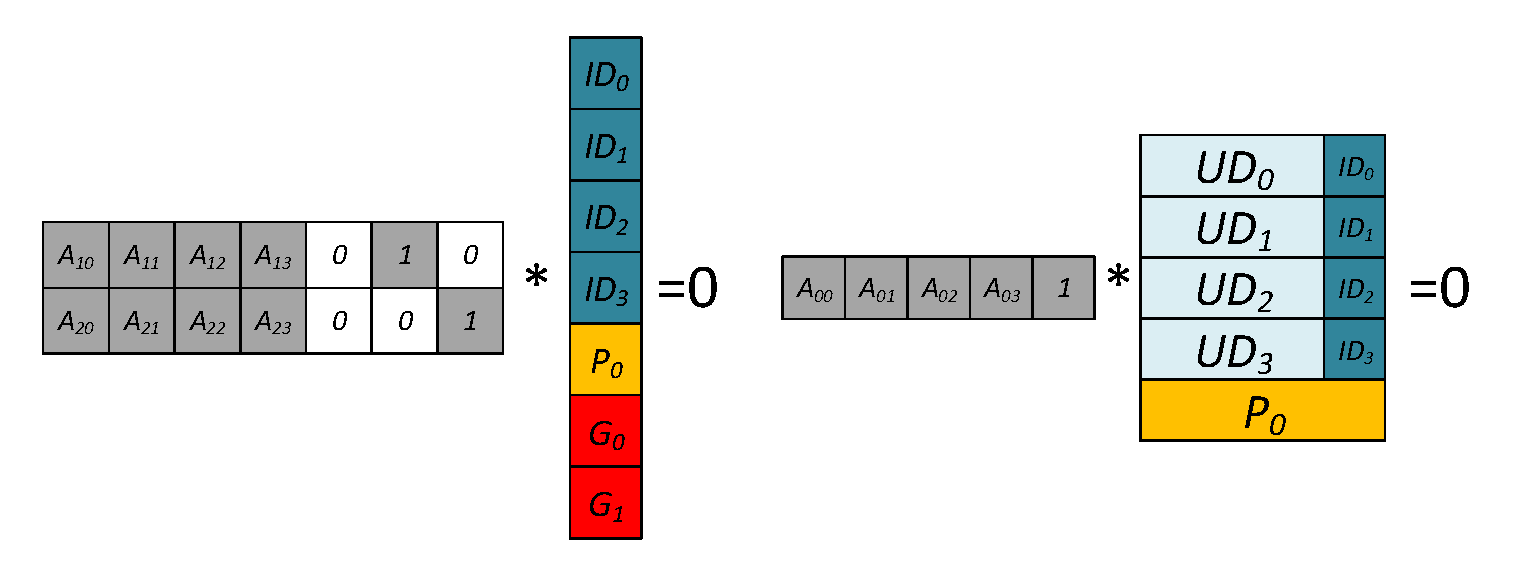
\includegraphics[width=0.45\textwidth]{photo/AP-RS-43.pdf}
\caption{The generate matrix of RS-based Approximate Codes $(4,1,4)$, where $ID_i$ and $UD_i$ represent the important and unimportant data in $N_i$. $G_0$ and $G_1$ are the parity blocks corresponding to important data blocks.}
\label{fig-ap-rs}
\end{figure}

\subsection{RS-based Approximate Code}
The construction of the Approximate Code based on RS is simple. In \emph{Structure 1}, the encoding unit is block. A horizontal RS parity is performed on the corresponding block in each chunk to generate a local parity block. At the same time, the important data blocks is horizontally verified by RS and generate multiple global check blocks.

In \emph{Structure 2}, the encoding unit is chunk.
We perform horizontal RS parity in each stripe to generate local parity chunks. The global parity chunk is generated only by the important data stripe.

Figure \ref{fig-ap-rs} is the RS generation matrix with $k=4$ and $r=1$.
It shows that to ensure that the coefficients of the local and the global parity are linearly independent is easy. If necessary, Approximation Code can easily achieve higher reliability guarantees based on RS, but in most cases this is excessive, so we will not discuss it here.

\subsection{XOR-based Approximate Code}
Since we mainly provide 3DFTs for important data, we prefer to construct Approximate Code with several RAID6-based codes to provide faster encoding and reconstruction speed than RS. This section introduce tipical cases of the construction of XOR-based Approximate Code ($5,1,6$, \emph{Structure 1}) and ($4,2,4$, \emph{Structure 2}).

\subsubsection{RAID5-TIP Approximate Code}
\begin{figure}[h]
\centering
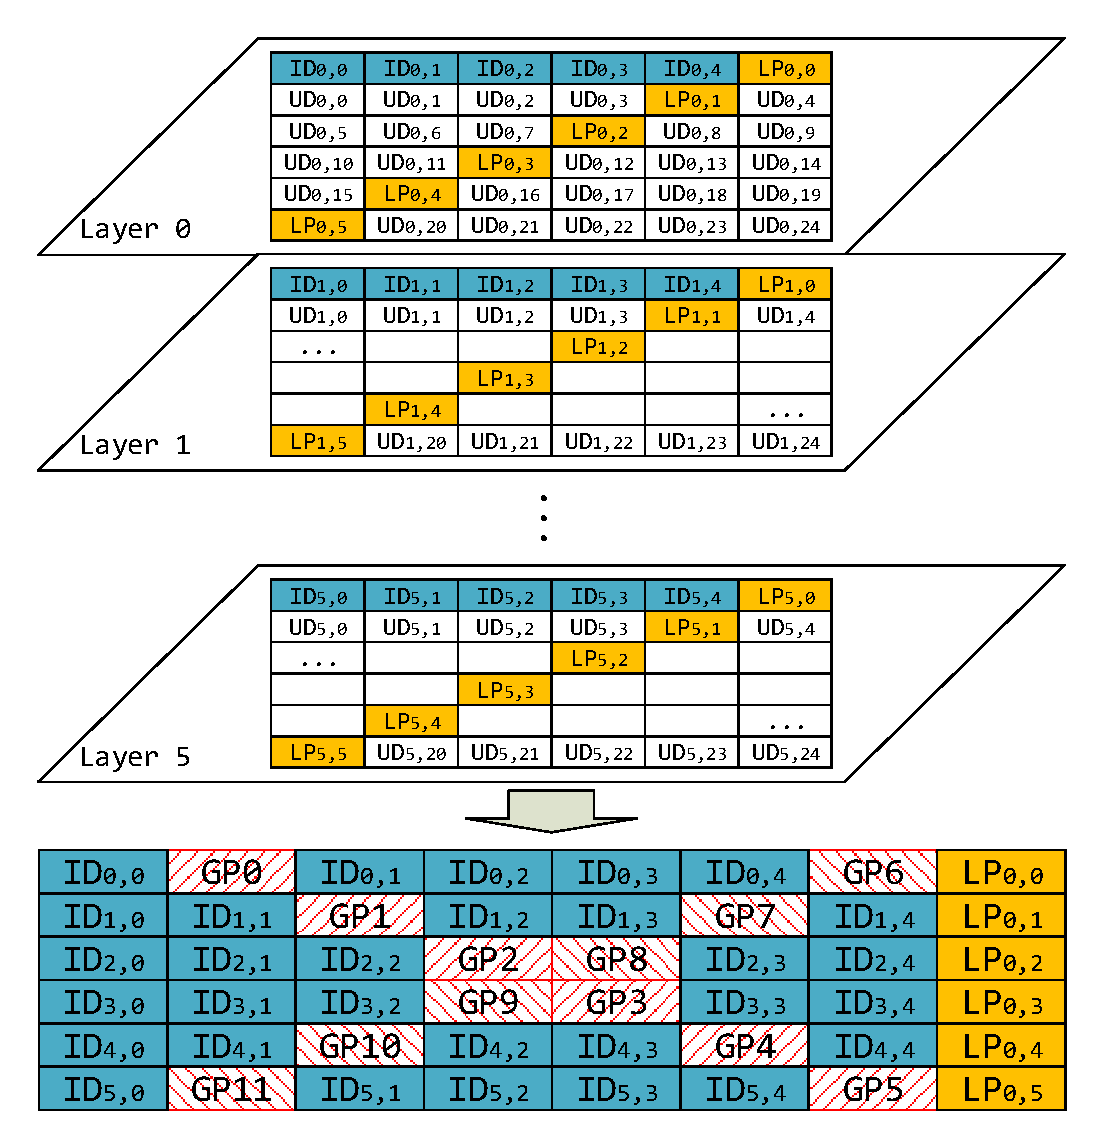
\includegraphics[width=0.35\textwidth]{photo/AP-TIP-v2.pdf}
\caption{The XOR-based Approximate Code ($5,1,6$, \emph{Structure 1}), constructed based on RAID5 and TIP-code.}
\label{fig-ap-TIP}
\end{figure}

Figure \ref{fig-ap-TIP} is a tipical construction of Approximate Code ($5,1,6,6$) in \emph{Structure 1}, based on RAID5 and TIP-code \cite{zhang2015tip}. RAID5 tolerate one node failure while TIP-code is an XOR-based 3DFTs code. In each stripe, local parity blocks provide horizontal XOR parity, and between stripes, global parity provide diagonal parity and anti-diagonal parity. 

The local (horizontal) parity elements are calculated by the following encoding equations.
\begin{align}
    LP_{i,0} &= \bigoplus_{j=0}^{k-1} ID_{i,j} (0 \leqslant i < h)\\
    LP_{i,p}(0<p<s) &= \bigoplus_{j=k(p-1)}^{kp-1} UD_{i,j} (0 \leqslant i < h)
\end{align}

When generating global parity blocks, the important data block, the local parity block, and the global parity block should be arranged as the encoding form of TIP-code. Figure \ref{fig-TIP} shows the coding method of diagonal and anti-diagonal parity blocks.
Since the encoding process of important data blocks can be seen as RAID5 plus TIP-code, it is obvious that they achieve 3DFTs.

\begin{figure}[h]
\subfigure[Diagonal parity $GP_0$ to $GP_5$, (e.g., $GP_0=ID_{0,0} \oplus ID_{1,4} \oplus ID_{2,3} \oplus ID_{4,2} \oplus ID_{5,1}$]{
    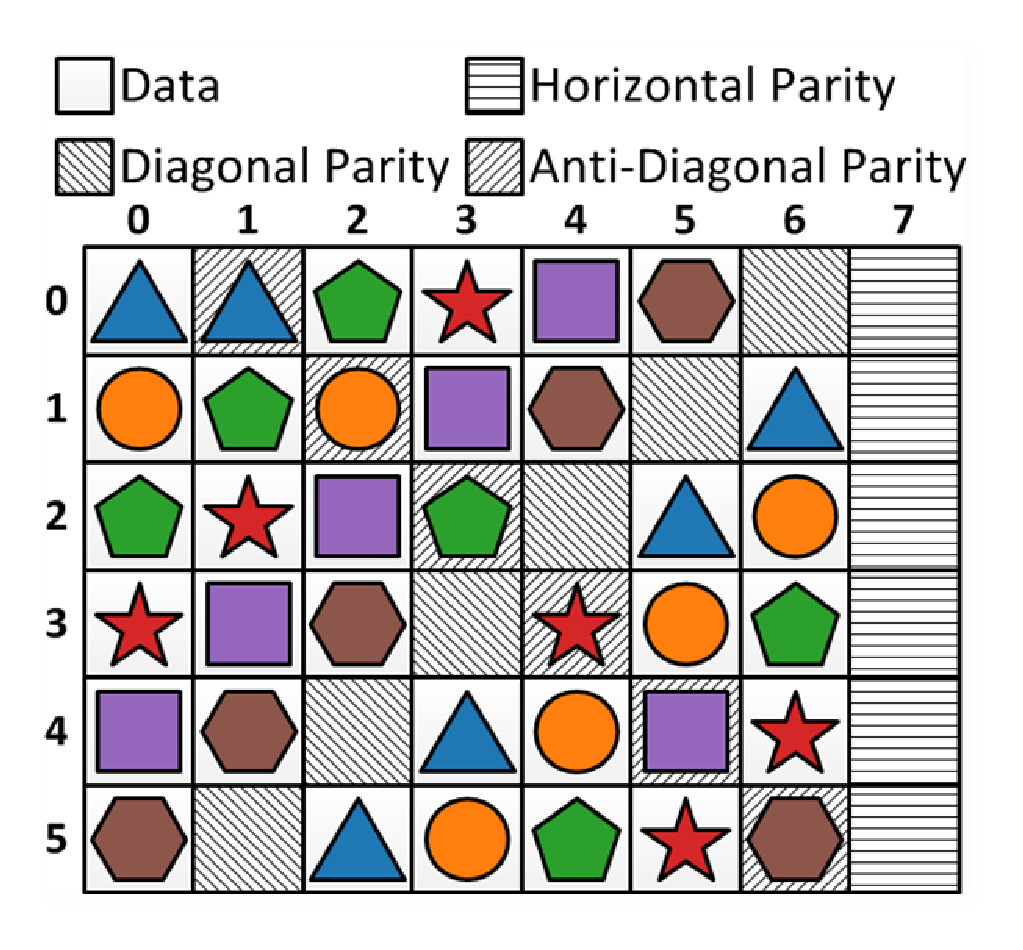
\includegraphics[width=0.2\textwidth]{photo/TIP-diag.pdf}
}
\subfigure[Anti-diagonal parity $GP_6$ to $GP_{11}$, (e.g., $GP_7=ID_{0,0} \oplus ID_{1,1} \oplus ID_{2,2} \oplus ID_{4,3} \oplus ID_{5,4}$)]{
    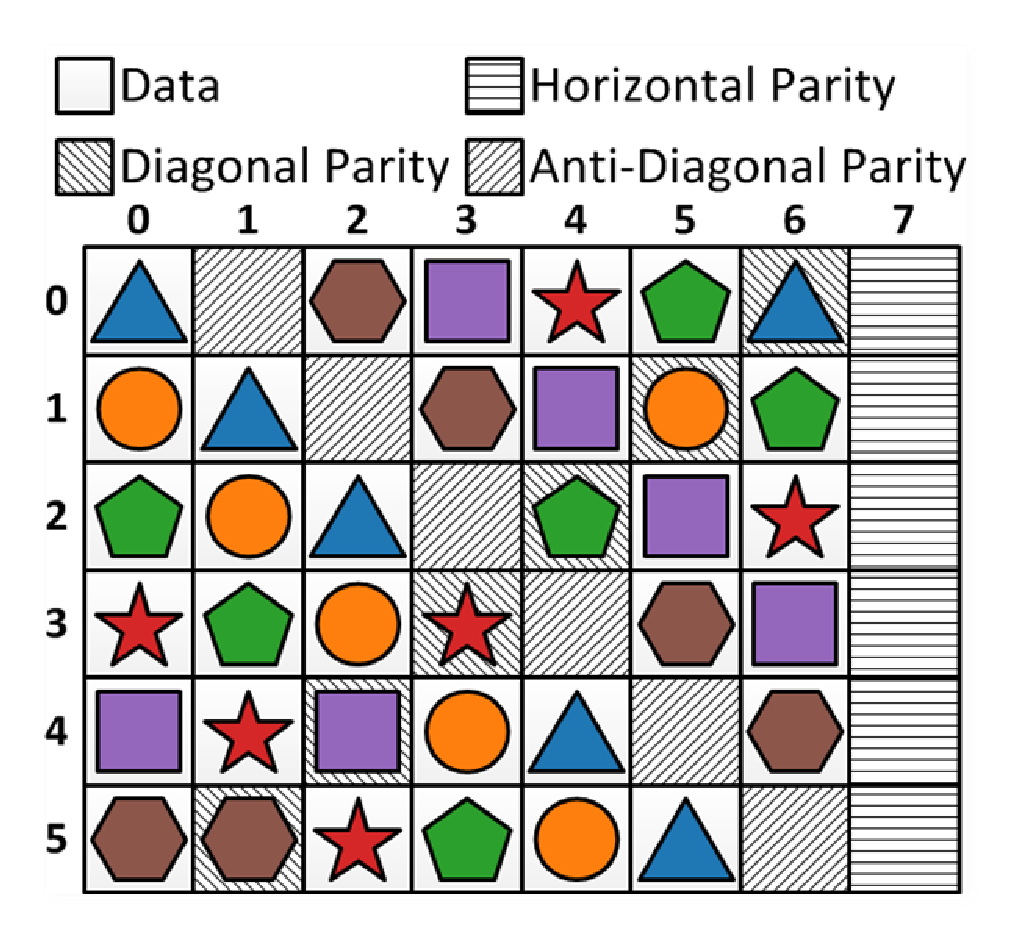
\includegraphics[width=0.2\textwidth]{photo/TIP-anti-diag.pdf}
}
\caption{Encoding pf TIP-code}
\label{fig-TIP}
\end{figure}

\subsubsection{EVENODD-STAR Approximate Code}
Figure \ref{fig-ap-STAR} shows the construction of Approximate Code ($4,2,4$) in \emph{Structure 2} based on EVENODD \cite{blaum1995evenodd} and STAR \cite{huang2008star}. 
EVENODD is a tipical RAID6 erasure code scheme, while STAR is a 3DFTs extension scheme of EVENODD. In this case, important data blocks are distributed in stripe 0, while unimportant data blocks occupy the rest stripes. 
Because the STAR code is constructed just by adding a reverse parity chain to the EVENODD code. In this case, we design a global parity block to store this parity chain, so 3DFTs can be guaranteed.

\begin{figure}[h]
\centering
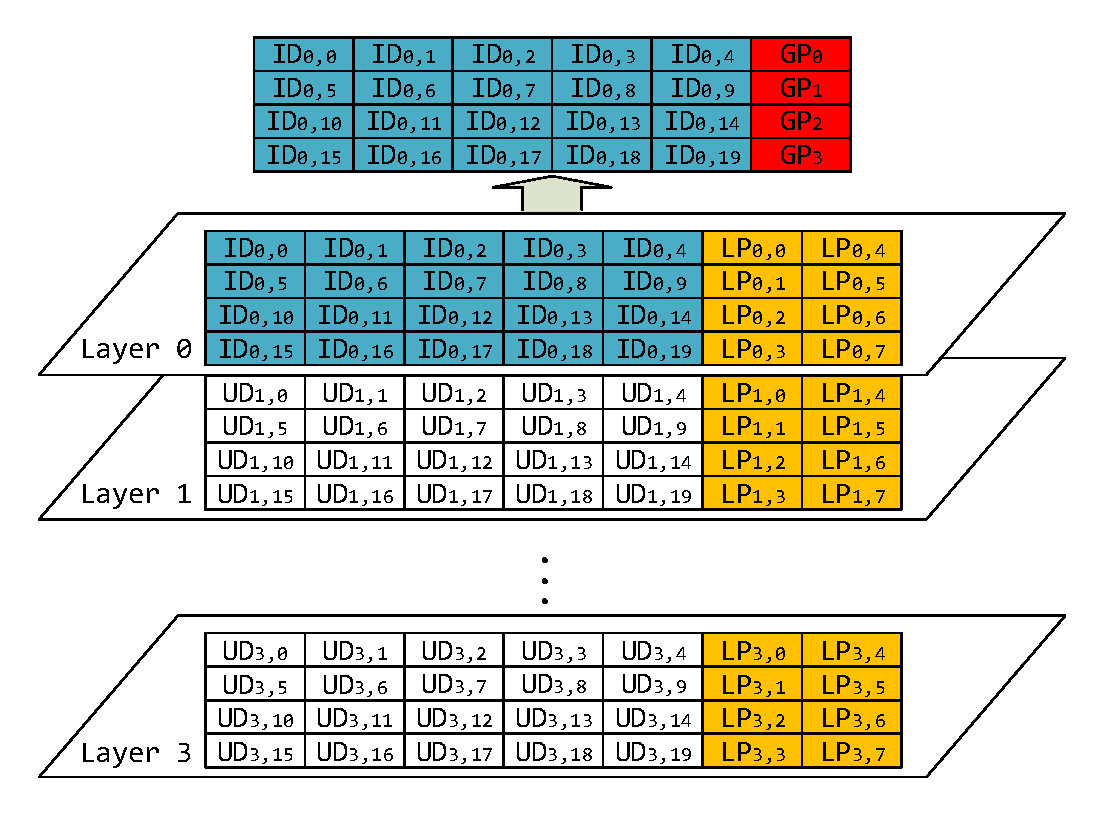
\includegraphics[width=0.35\textwidth]{photo/AP-EVEN-star-v2.pdf}
\caption{The XOR-based Approximate Code ($4,2,4,4$), constructed based on EVENODD and STAR code. $LP$ represent the local parity and $GP$ represent the global parity.}
\label{fig-ap-STAR}
\end{figure}

\subsection{Decoding Case Study}
This section describe the decoding methods in different cases of node failure based on \emph{Structure 1} and \emph{Structure 2}.

\subsubsection{Reconstruction cases in Structure 1}
Under \emph{Structure 1}, important data and unimportant data are distributed in 

\subsubsection{Reconstruction cases in Structure 2}

\subsection{Properties of Approximate Code}

We analyze the nature of the Approximate Code from the following aspects, and the calculation method of the relevant indicators is given in Table \ref{tab-AS-RS-AP}.
\begin{itemize}
    \item Low Storage Overhead: Approximate Code reduces storage overhead by approximating storage strategies. This property is more pronounced for data with a smaller proportion of important data.
    \item Low Update Overhead: When one node is updated, Approximate Code only needs to write $r \times h$ local parity chunks and only $3-r$ global parity chunks, while tipical 3DFTs EC methods should write $3 \times h$ parity chunks.
    \item High reliability for important data. The Approximate Code guarantees 3DFTs for important data.
    \item Flexibility. The implementation of the Approximate Code can be based on RS, XOR or a mixture of the two.
\end{itemize}

\begin{table}[ht]
\centering 
\caption{Comparison of storage overhead and fault tolerance between Ap-Code (short for Approximate Code), RS and several XOR-based codes.}\label{tab-AS-RS-AP}
\begin{tabular}{|c|c|c|c|}
\hline
EC & \begin{tabular}[c]{@{}c@{}}Storage\\ Overhead\end{tabular} & \begin{tabular}[c]{@{}c@{}}Fault \\ Tolerance\end{tabular} & \begin{tabular}[c]{@{}c@{}}Single Node\\Update Cost\end{tabular} \\ \hline
RS($k,r$) & $(k+r)/k$ & $r$ & r \\ \hline
EVENODD($k,2$) & $(k+2)/k$ & 2 & 2 \\ \hline
TIP-code/STAR($k,3$) & $(k+r)/k$ & 3 & 3 \\ \hline
\begin{tabular}[c]{@{}c@{}}Ap-Code\\ ($k,r,h$)\end{tabular} & $\frac {(k+r)h+3-r}{k \times h}$ & r to 3 & $r+\frac{3-r}{h}$ \\ \hline
\end{tabular}
\end{table}

\section{Implementation}\label{Implementation}
\begin{figure}[htb]
\centering
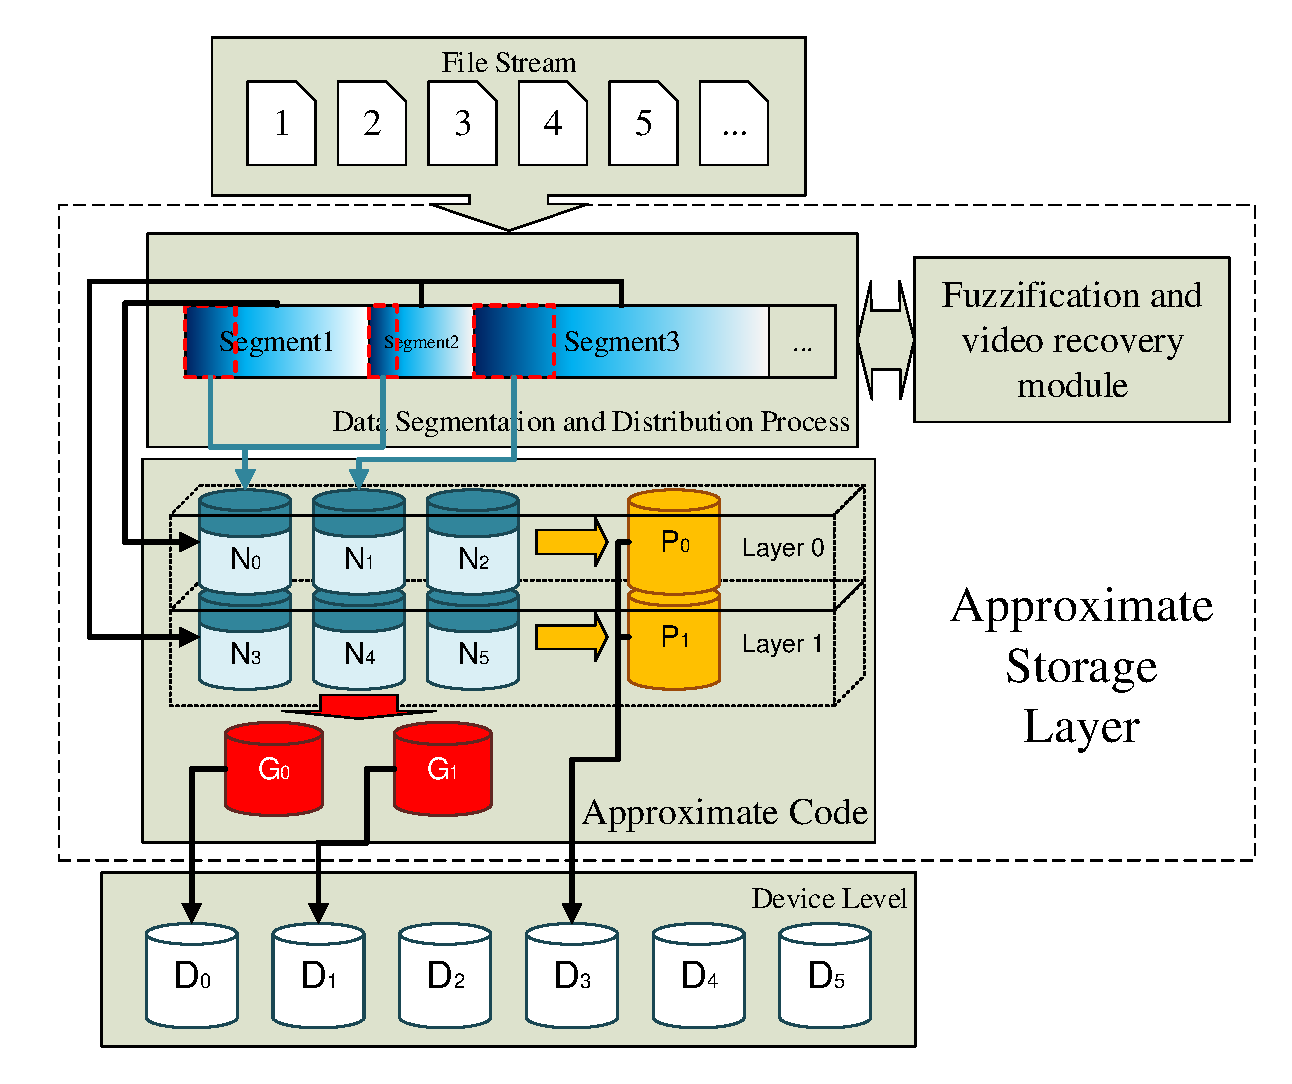
\includegraphics[height = 6.5cm]{photo/implementation-V2.pdf}
\caption{Overview of Approximate Code implementation}
\label{fig-implementation}
\end{figure}

Compared with the traditional scheme that does not consider the meaning of the upper stripe data, the Approximate Code pays attention to the difference of the importance of the data, so an intermediate stripe between the upper stripe application and the underlying distributed storage system is necessary to preprocess the data. We call it the approximate storage stripe, which include 3 parts: data identification and allocation, encoding and decoding process of Approximate Code and the video fuzzification and recovery.

\subsection{Data Segmentation and Distribution module}
The data segmentation module splits the video file stream into multiple data segments and automatically discriminates the important data. A natural approach is to follow the GOP segmentation. According to the \ref{video storage}, the GOP of the encoded video starts with an I frame, and all the data in that GOP depends on it for decoding, so we define it as important data and divide the GOP into I frames (important part) and other data. (unimportant part).

The data distribution module distributes important data and unimportant data in different blocks and records the location. This location information is also defined as important data. This module is also responsible for analyzing the proportion of important data and unimportant data in the data stream to select the most appropriate coding parameter configuration to ensure fault tolerance and high storage efficiency of important data.

\subsection{Approximate Code module}
The Approximate Code implements local and global encoding of $k*h$ data chunks and is responsible for reconstructing the wrong data chunk. When no more than $r$ chunks are corrupted, Approximation Code uses the local check block to recover all data, both important and minor. When there is no more than 3 loss of important data,
2 forms
Form 1: Important data and unimportant data are distributed at the same node.
When there are no more than r blocks lost in a single stripe, the local check block completely recovers all data.
When more than r but no more than 3 blocks are lost in a single stripe, the global check block recovers all important data, and the surviving unimportant data block and important data blocks are sent to the video recovery module.
Form 2: The important data is distributed in a stripe, and the minor number is distributed on H-1 stripes. . .
Important data stripe loses no more than 3 blocks and is fully recovered.
The unimportant data stripe loses no more than r blocks and is fully recovered.
The unimportant data stripe loses more than r, and the video is restored.
The approximate code module is also responsible for allocating data blocks to ensure that the chunks of each stripe are distributed to different nodes, while ensuring that the global check chunk and the data chunk are not on one node.

\subsection{Data Fuzzification and Video Recovery}
In the approximate recovery mode, the recoverable and remaining data is passed to this module, and the blurred video is recovered through various video recovery techniques, and the upper application is notified. Through the content of the second chapter, we can approximate the data recovery. . .

\section{Approximate Recovery}\label{ap-recovery}

\begin{figure*}
\subfigure{
    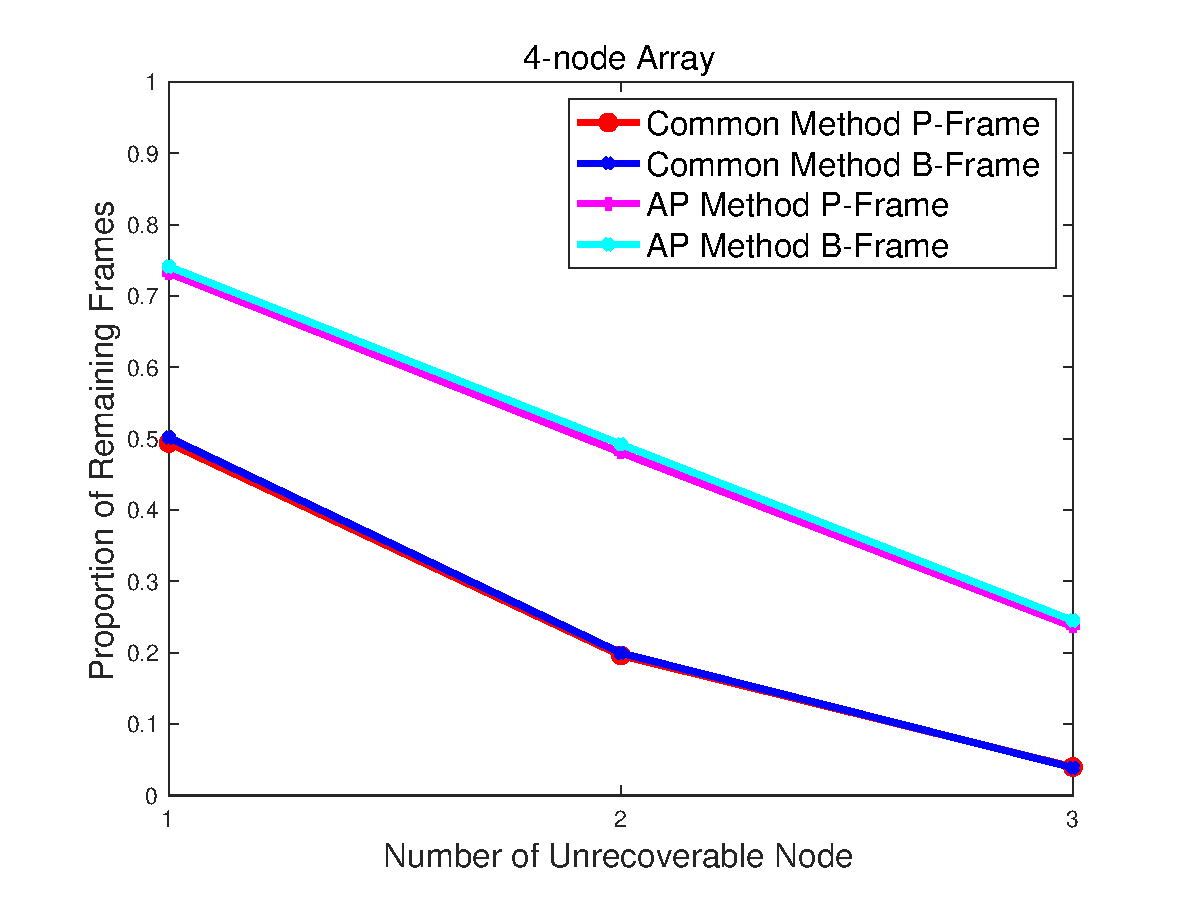
\includegraphics[width = 0.22\linewidth]{photo/experiment/Ap-recovery-4-disks.eps}
}
\subfigure{
    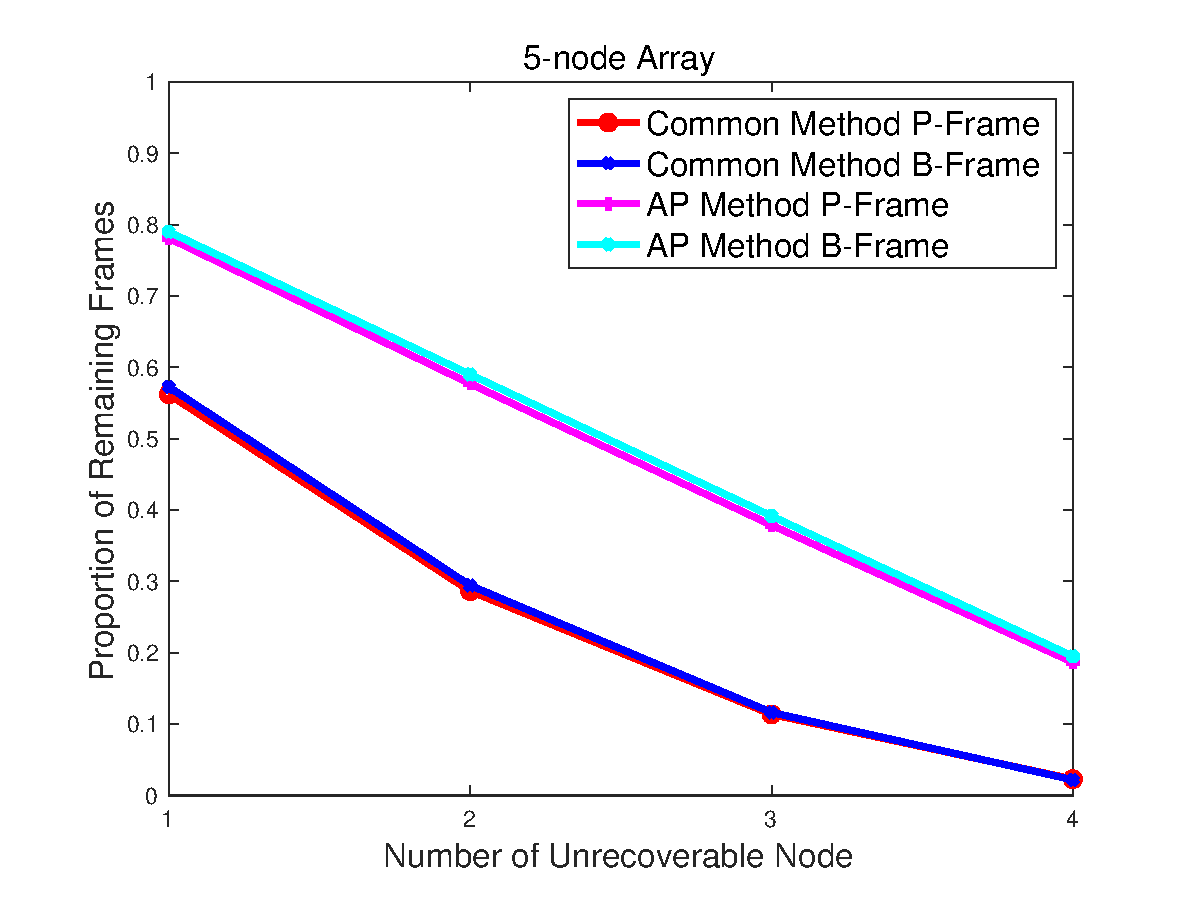
\includegraphics[width = 0.22\linewidth]{photo/experiment/Ap-recovery-5-disks.eps}
}
\subfigure{
    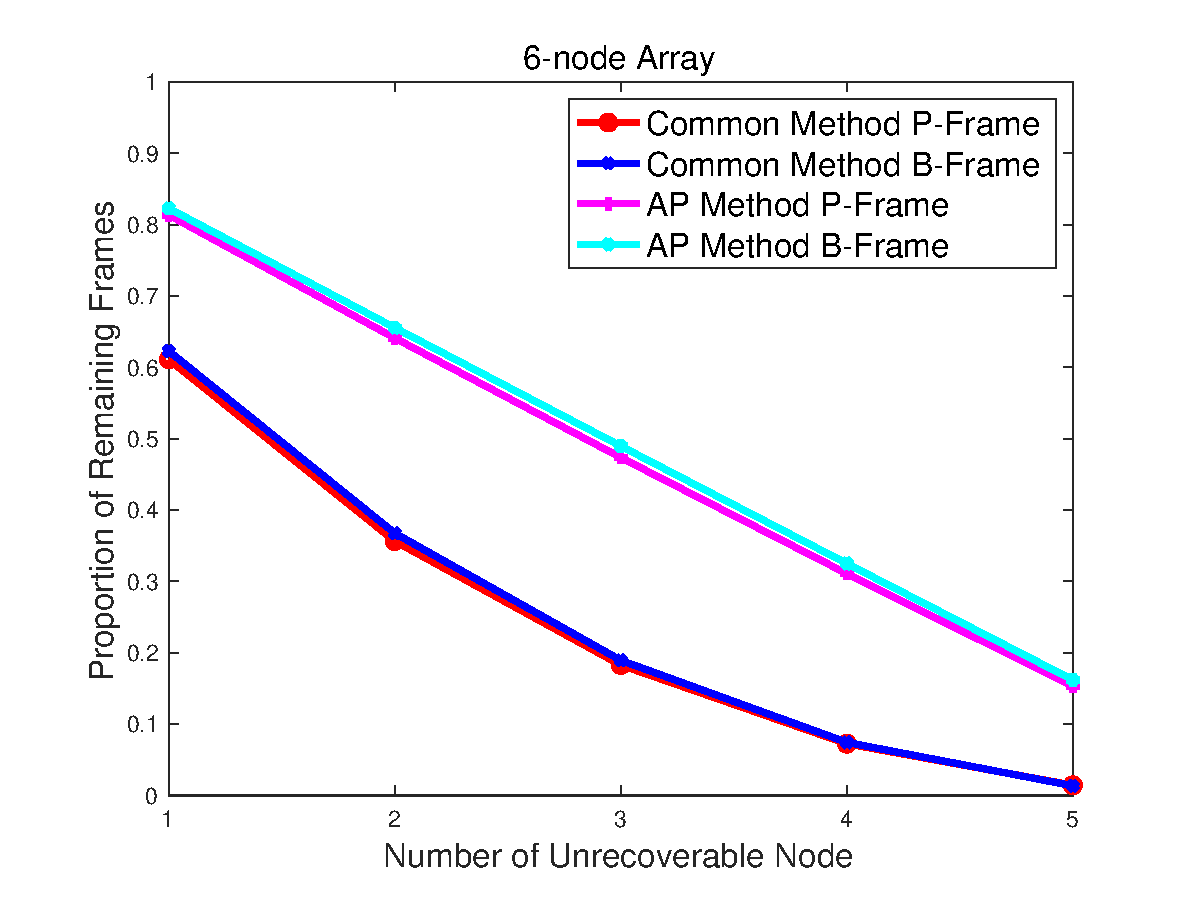
\includegraphics[width = 0.22\linewidth]{photo/experiment/Ap-recovery-6-disks.eps}
}
\subfigure{
    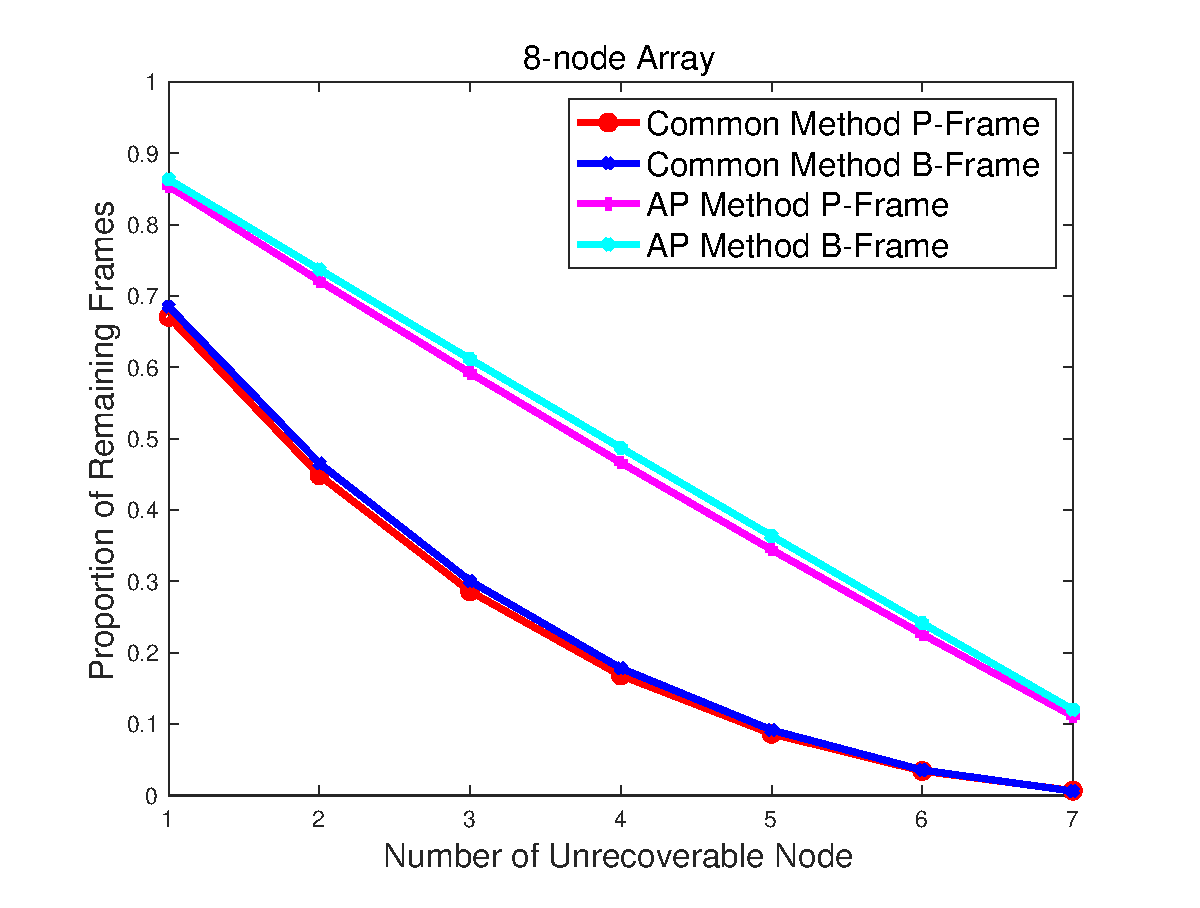
\includegraphics[width = 0.22\linewidth]{photo/experiment/Ap-recovery-8-disks.eps}
}
\caption{Comparison of the data retention  between approximate storage and common methods when node is unrecoverable.}
\end{figure*}


In this chapter, we mainly discuss the number of video frames saved in Mode 1 when the unimportant data corruption is greater than the fault tolerance of the local calibration and the important data can be fully recovered.
This proves that if the video data is not distinguished, in a typical
This compares the ability of the approximation code to secure video data.

Indicator: number of frames restored
Test situation:
Test set:

Our experiments analyzed a series of videos. We define that when the I frame of the video is corrupted, the entire GOP is marked as unavailable (lost).
Since the approximation code stores the I frame as important data, the integrity of the I frame is always guaranteed in our scheme.

The experimental results are shown in Figure x. The approximate storage scheme can guarantee the number of frames of the video close to the theoretical limit.


Our experiments prove that if data is stored indiscriminately, the loss of important data will seriously affect the security of all data, and our scheme will control the data loss near the theoretical limit, ensuring video recovery and fuzzification. feasibility.

\section{Evaluation}\label{evaluation}

Storage overhead

Encoding and decoding performance

write performance

recovery Overhead

Recovery Frame


Our experiment is mainly divided into two parts: erasure code and approximate storage analysis. The former mainly analyzes the performance of the approximate code and compares our scheme with the typical erasure code configuration; the latter mainly analyzes the data protection capability of the approximate code and other schemes in the case of data loss.



In this section, we use mathematical analysis and a series of experiments to demonstrate the performance of the approximate code.
Evaluation method: We choose RS code, TIP-code, EVENODD, STAR, RAID5 for comparison.

Mathematical analysis: We use the storage efficiency, fault tolerance and reconstruction cost defined above as a measure.

In short, for each stripe, the unimportant data can tolerate any r node failures, while important data can tolerate any three node failures. However, the actual scene will be more complicated:
For mode one. . .


For fault tolerance, Mode 1 and Mode 2 will be different. Not only that, Mode 1 provides minimal fault tolerance, while Mode 2 provides near-code maximum fault tolerance.

Obviously, for mode one, the approximate code can tolerate any r node failures, and the fault tolerance of important data is 3. For mode two, the approximate code provides an arbitrary level of r-node failure, and only if

For mode two, if all chunks are distributed across different nodes, the approximate code provides the greatest degree of reliability. That is,



We calculated the recovery efficiency and reconstruction cost of the approximate code in the case of single-node, two-node and three-node failures. Since the approximate code can be constructed in many forms, we mainly focus on it. . . . . .




\section{Conclusion}\label{Conclusion}

\textcolor{gray}{
    text text text text text text text text text text text text text text text text text text text text text text text text text text text text text text text text text text text text text text text text text text text text text text text text text text text text text text text text text text text text text text text text text text text text text text text text text text text text text text text text text text text text text text text text text text text text text text text text text text text text text text text text text text text text text text text text text text text text text text text text text text text text text text text text text text text text text text text text text text text text text text text text text text text text text text text text text text text text text text text text text text text text text text text text text text text text text text text text text text text text text text
    text text text text text text text text text text text text text text text text text text text text text text text text text text text text text text text text text text text text text text text text text text text text text text text text text text text text text text text text text text text text text text text text text
}


\begin{acks}

\end{acks}



\bibliographystyle{ACM-Reference-Format}
\bibliography{ApproximateCode}

\end{document}
